\documentclass{article}

% Import packages from local file
\usepackage{packages}

% Define the homework number as a variable
\newcommand{\HomeworkNumber}{5}

\begin{document}

% Add the cover


% Set up custom date format
\newdateformat{monthyeardate}{\monthname[\THEMONTH] \THEYEAR}

% Header and Footer configuration
\pagestyle{fancy}
\fancyhf{}
\fancyhead[L]{\leftmark}
\fancyhead[R]{\thepage}
\fancyfoot[C]{Probabilistic Modeling and Reasoning Homework \HomeworkNumber}

% Chapter and Section formatting
\titleformat{\chapter}[display]
  {\normalfont\bfseries}{}{0pt}{\Huge}
\titlespacing*{\chapter}{0pt}{-20pt}{20pt}

% Adjust header height and top margin
\setlength{\headheight}{14.49998pt}
\addtolength{\topmargin}{-2.49998pt}

% Custom abstract environment
\newenvironment{customabstract}
  {\vspace*{1cm}
   \begin{center}
   \bfseries \huge Abstract
   \end{center}
   \vspace{0.5cm}
   \normalfont \large}
  {\vspace{1cm}}



\makeatletter
% Taken from http://ctan.org/pkg/centernot
\newcommand*{\centernot}{%
  \mathpalette\@centernot
}
\def\@centernot#1#2{%
  \mathrel{%
    \rlap{%
      \settowidth\dimen@{$\m@th#1{#2}$}%
      \kern.5\dimen@
      \settowidth\dimen@{$\m@th#1=$}%
      \kern-.5\dimen@
      $\m@th#1\not$%
    }%
    {#2}%
  }%
}
\makeatother


\begin{titlepage}
    \centering

    % University logo
    \vfill
    
\includegraphics[width=0.3\textwidth]{UOMLOGOEN.eps}
    \vfill

    % Main title
    {\Huge \textbf{Probabilistic Modeling and Reasoning}} \\
    {\LARGE Homework — \HomeworkNumber}

    \vfill  % Vertical fill for dynamic centering
    % Authors' names
    {\Large \textbf{Nikolaos Liouliakis (AID25001)}} \\
    {\Large \textbf{Vasileios-Efraim Tsavalia (AID25006)}}

    % \vfill

    % % Course submission information
    % {\Large A report submitted for the course} \\
    % {\Large \textbf{Probabilistic Modeling and Reasoning}}

    \vfill

    % Program and University information
    {\Large MSc in Artificial Intelligence and Data Analytics} \\
    {\Large University of Macedonia}

    \vfill


    % Supervisor information
    {\Large \textbf{Supervisor: Professor Dimitris Christou-Varsakelis}}

    \vfill

    % Date with custom format
    {\Large \monthyeardate\today} % Automatically displays in "October 2024" format
    
\end{titlepage}


\newpage



\section*{Problem 1}

After renaming the variables as following, the probability we want to calculate is:



\begin{table}[H]
\centering
\begin{tabular}{|c|c|}
\hline
\textbf{Old variable name} & \textbf{New variable name} \\ \hline
fuse assembly malfunction & $x_0$ \\ \hline
drum unit                 & $x_1$ \\ \hline
toner out                 & $x_2$ \\ \hline
poor paper quality        & $x_3$ \\ \hline
worn roller               & $x_4$ \\ \hline
burning smell             & $x_5$ \\ \hline
poor print quality        & $x_6$ \\ \hline
wrinkled pages            & $x_7$ \\ \hline
multiple pages fed        & $x_8$ \\ \hline
paper jam                 & $x_9$ \\ \hline
\end{tabular}
\caption{Mapping of original variable names to new variable names.}
\label{tab:my-table}
\end{table}

\[
p(x_1 = 1 \mid x_7 = 0 , x_5 = 0 , x_3 = 1 ) = 0.5075
\]

It was calculated in python utilizing the "pyAgrum" library in the Python script named \textit{Problem1\_EM.py}


\section*{Problem 2}

The Python script is named \textit{Gaussian\_Mixture.py} and generates the output file named \textit{em\_output.txt} 


% https://www.wolframalpha.com/input?i=log%281%2F%282*sqrt%28pi%29%29+*+%28e%5E%28-%282.75-x%29%5E2%29+%2Be%5E%28-%282.75-2*x%29%5E2%29%29%29


\section*{Problem 3} 

The marginal likelihood is determined by summing over \(x_2\):
\[
p(x_1 = i) = \sum_{j=1}^{2} \theta_{ij}.
\]

1. For the first matrix:
\[
\theta^{(1)} =
\begin{pmatrix}
0.3 & 0.3 \\
0.2 & 0.2
\end{pmatrix}
\]
we compute:
\[
p(x_1 = 1) = \theta_{11} + \theta_{12} = 0.3 + 0.3 = 0.6, \quad 
p(x_1 = 2) = \theta_{21} + \theta_{22} = 0.2 + 0.2 = 0.4.
\]

2. For the second matrix:
\[
\theta^{(2)} =
\begin{pmatrix}
0.2 & 0.4 \\
0.4 & 0
\end{pmatrix}
\]
we compute:
\[
p(x_1 = 1) = \theta_{11} + \theta_{12} = 0.2 + 0.4 = 0.6, \quad 
p(x_1 = 2) = \theta_{21} + \theta_{22} = 0.4 + 0 = 0.4.
\]

Since the marginal probabilities \(p(x_1 = i)\) are identical for both matrices (\(p(x_1 = 1) = 0.6\) and \(p(x_1 = 2) = 0.4\)), both \(\theta^{(1)}\) and \(\theta^{(2)}\) yield the same marginal likelihood score.



\section*{Problem 4}

Output of the "EM" function (implemented in \textit{EM.m}) for input EM(1.9,0.2), where 1.9 is the starting value for $\theta$ and 0.2 is the starting value for $q(h=2)$.

\begin{figure}[H]
    \centering
    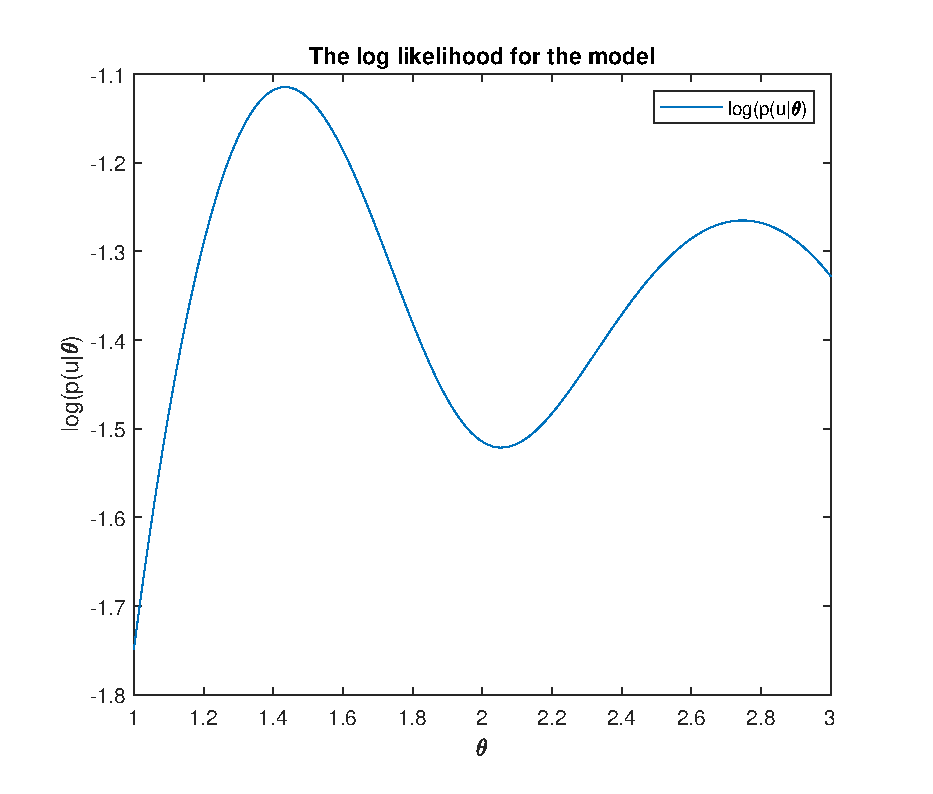
\includegraphics[width=0.8\textwidth]{log_likelihood.eps} % Replace with your EPS file name
    \caption{The log likelihood}
    % \label{fig:eps-figure}
\end{figure}

\begin{figure}[H]
    \centering
    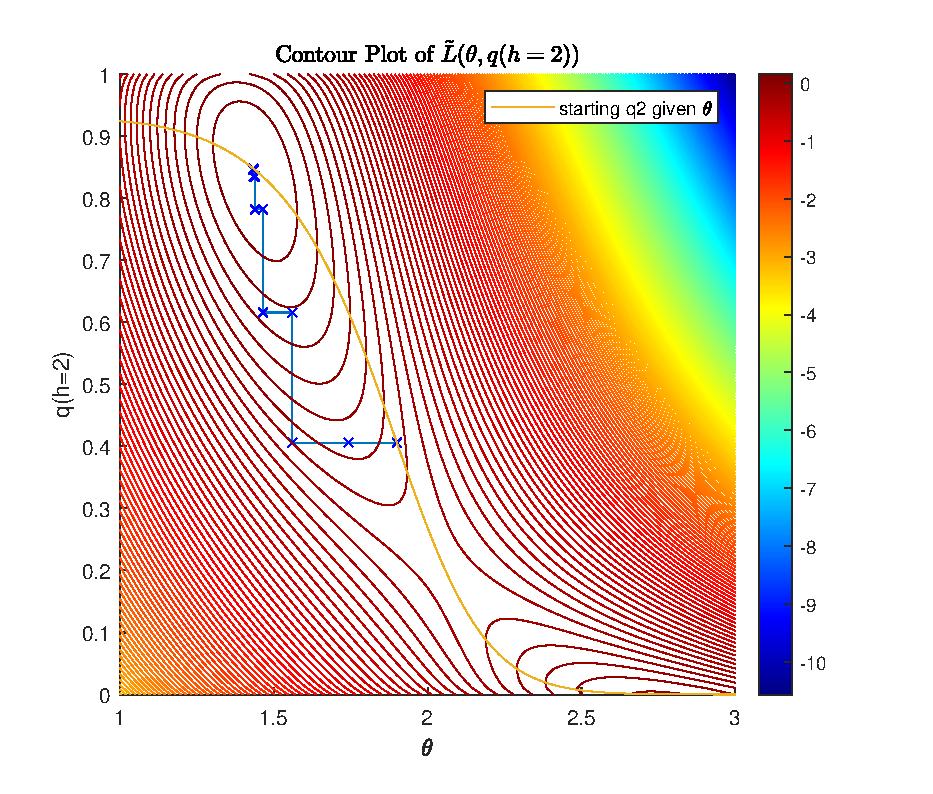
\includegraphics[width=0.7\textwidth]{converging_EM1.eps} % Replace with your EPS file name
    \caption{Convergence using 1.9 for the starting value for $\theta$ }
    % \label{fig:eps-figure}
\end{figure}

\begin{figure}[H]
    \centering
    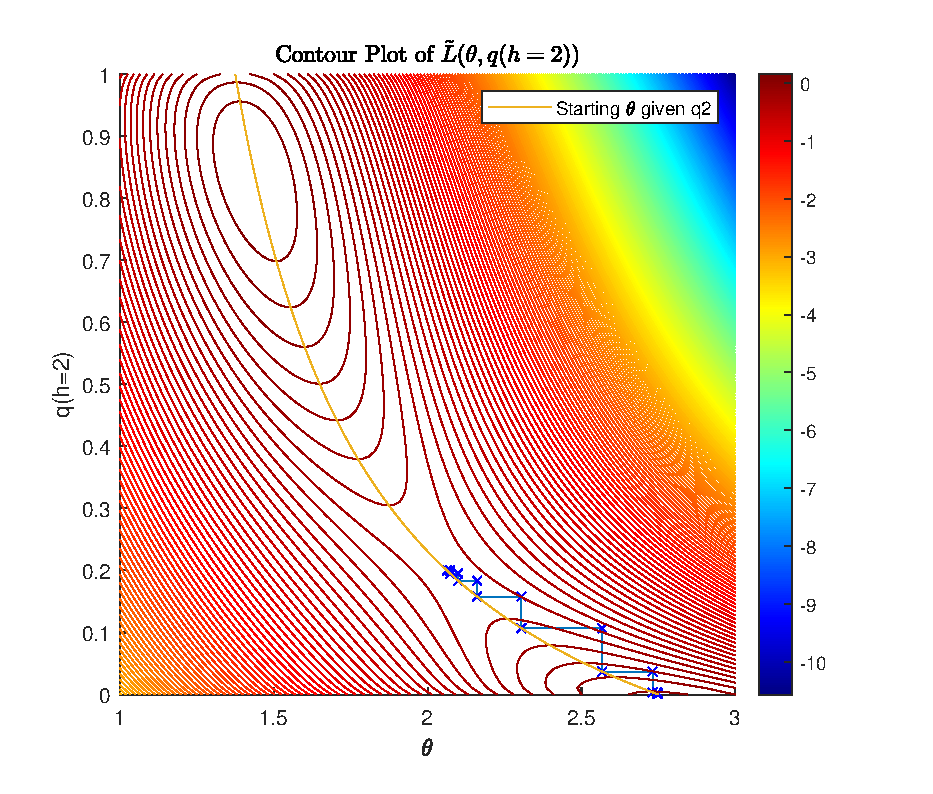
\includegraphics[width=0.7\textwidth]{converging_EM2.eps} % Replace with your EPS file name
    \caption{Convergence using 0.2 for the starting value for $q(h=2)$ }
    % \label{fig:eps-figure}
\end{figure}

\end{document}
